% RehaPiano – testy EXACT_FORCE a rytmus: hypotézy, normy, klasifikátor, porovnanie
% Kompilácia: pdflatex dokumentacia.tex (2x), tectonic dokumentacia.tex, alebo nahrať celý priečinok docs/latex do Overleafu.
\documentclass[11pt,a4paper]{article}

\usepackage{iftex}
\ifXeTeX
  \usepackage{fontspec} % XeTeX / tectonic: Unicode fonts (Latin Modern)
\else
  \usepackage[utf8]{inputenc}
  \usepackage[T1]{fontenc}
  \usepackage{lmodern}
\fi
\usepackage[slovak]{babel}
\usepackage[a4paper,margin=2.2cm]{geometry}
\usepackage{amsmath,amssymb}
\usepackage{graphicx}
\usepackage{booktabs}
\usepackage{tabularx}
\usepackage{array}
\usepackage{enumitem}
\usepackage{float}
\usepackage[hidelinks]{hyperref}
\usepackage{url}

\graphicspath{{obrazky/}}
\setlist{itemsep=2pt,topsep=4pt}
\setlength{\parskip}{4pt}
\setlength{\parindent}{0pt}
\setlength{\emergencystretch}{2em} % long words like EXACT_FORCE cannot be hyphenated
\renewcommand{\arraystretch}{1.15}
\newcolumntype{L}{>{\raggedright\arraybackslash}X}
\newcommand{\ok}{\checkmark}
\newcommand{\ef}{EXACT\_FORCE}
\newcommand{\yes}{\textbf{potvrdená}}
\newcommand{\no}{nepotvrdená}

\title{RehaPiano -- testy \ef{} a rytmus:\\ hypotézy, normy, klasifikátor a porovnanie testov}
\author{Maksym Kuznietsov \and Dmytro Sholtys \and Mykyta Holovcyk}
\date{}

\begin{document}
\maketitle

\noindent\textbf{Obsah:} štatistická analýza dvoch testov RehaPiana -- \ef{} a rytmického testu (hypotézy,
zmeny s~vekom a~normy, klasifikátor, ablácia), porovnanie ich záverov a~diskusia.

% ===================================================================================================
\section{Dáta a testy}

\begin{table}[H]
\centering
\begin{tabular}{lcc}
\toprule
 & zdraví & pacienti \\
\midrule
počet osôb & \textbf{135} & \textbf{48} \\
vek -- medián (rozsah) & 61 (18 -- 85) & 66,5 (21 -- 89) \\
osoby nad 50 rokov & 74 & 40 \\
\bottomrule
\end{tabular}
\end{table}

\begin{itemize}
  \item \textbf{Zdraví} = osoby, ktoré v~dotazníku neuviedli žiadne ochorenie (135 zo 167 zdravých). Normálne hodnoty
        musia byť z~naozaj zdravých ľudí. Kontrola so všetkými 167 zdravými dáva takmer rovnaké závery.
  \item \textbf{Odkiaľ sú zdraví:} mladí z~meraní TUKE (2025), starší väčšinou z~meracieho centra (9.~9.~2026
        a~9.~--~13.~11.~2026; 59 zdravých bez ťažkostí z~novembra). Pacienti sú zatiaľ len tí s~metadátami
        (nové merania pacientov z~roku 2026 ešte nemajú vek a~pohlavie, preto nie sú zahrnuté).
  \item Tí istí ľudia urobili oba testy. \textbf{35 pacientov} bolo meraných dvakrát (medián 7 dní medzi meraniami).
  \item \textbf{Pozor:} pacienti sú starší (medián 66,5 vs. 61 rokov) a~mladší zdraví sú z~iného miesta merania ako
        starší. Preto každý rozdiel kontrolujeme aj pri rovnakom veku.
  \item RehaPiano má 10 snímačov sily (5 prstov $\times$ 2 ruky); signál sa prevzorkuje na 100~Hz (krok 10~ms).
\end{itemize}

\textbf{Dva testy:}
\begin{itemize}
  \item \textbf{\ef{}} -- osoba drží všetkými prstami rovnomernú silu, 4 pokusy po 16~s.
        Meria \textbf{tras a~stabilitu sily}.
  \item \textbf{Rytmický test (RHYTHM)} -- osoba čo najrýchlejšie rytmicky stláča a~uvoľňuje obomi rukami naraz,
        4 pokusy po 31~s. Meria \textbf{rýchlosť, koordináciu a~rovnováhu rúk}.
\end{itemize}
V~oboch testoch je \textbf{1. pokus nácvik} (človek si zvyká na hru a~prístroj) a~nepoužíva sa; analyzujú sa
pokusy 2 -- 4.

% ===================================================================================================
\section{Metodika (rovnaká pre oba testy)}

Pre každý test vypočítame 10 parametrov osoby, rozdelených do 8 skupín (\textbf{faktorov}). Oba testy potom
prejdú rovnakým postupom (spoločný kód \path{src/rehapiano/common/stats/group_analysis.py}), aby sa výsledky dali
porovnať.

\textbf{1. Hypotézy a~testy.} Pre každý parameter: \textbf{H0} -- zdraví a~pacienti majú rovnaké rozdelenie;
\textbf{H1} -- u~pacientov je parameter vyšší / nižší (smer je pri každom parametri v~tabuľke hypotéz). Rozdiel
kontrolujeme v~štyroch krokoch, od najjednoduchšieho po najprísnejší:
\begin{enumerate}
  \item \textbf{Mann-Whitneyho test}, všetci zdraví vs. všetci pacienti (neparametrický -- parametre nemajú
        normálne rozdelenie). \textbf{AUC} = pravdepodobnosť, že náhodný pacient má vyššiu hodnotu ako náhodný
        zdravý (0,5 = žiadny rozdiel).
  \item \textbf{Rovnako starí:} Mann-Whitney v~každej dekáde, spojený do jedného testu (\textbf{van Elterenov test}).
  \item \textbf{Lineárny model} parameter = $b_0 + b_{\text{vek}}\cdot\text{vek} + b_{\text{ochorenie}}\cdot\text{pacient}$
        -- vplyv ochorenia pri rovnakom veku.
  \item Ten istý model s~ďalšou premennou, ktorá môže rozdiel vysvetliť: v~\ef{} \textbf{sila prstov}
        (tras rastie so silou), v~rytme \textbf{tempo} (pomalé stláčanie mení silu aj uvoľnenie).
\end{enumerate}
Testujeme 10 parametrov naraz, preto p-hodnoty opravujeme \textbf{Holmovou korekciou} (bez nej by pri 10 testoch
vyšiel aspoň jeden \uv{významný} rozdiel náhodou s~pravdepodobnosťou približne 40\,\%).
Hypotéza je \textbf{potvrdená}, ak je rozdiel významný ($p < 0{,}05$ po korekcii) v~očakávanom smere aj
\textbf{pri rovnakom veku} (krok 2).

\textbf{2. Vek a~normy.} Iba zdraví: \textbf{H0} -- parameter nesúvisí s~vekom (Spearmanova korelácia, Holmova
korekcia). Norma = medián a~rozsah 2,5. -- 97,5. percentil zdravých (rozsah, v~ktorom je 95\,\% zdravých).
Zdravých v~dekádach (10 -- 19 \dots{} 80 -- 89) je 8 / 43 / 4 / 5 / 7 / 33 / 34 / 1; spoľahlivý rozsah potrebuje
aspoň približne 20 osôb, čo majú dekády 20 -- 29, 60 -- 69 a~70 -- 79. Preto normu počítame zo všetkých zdravých naraz:
\begin{itemize}
  \item parameter \textbf{bez vplyvu veku} $\Rightarrow$ rovnaká norma pre všetky dekády;
  \item parameter \textbf{s~vplyvom veku} $\Rightarrow$ kvantilová regresia na vek (hranice normy sa menia s~vekom).
\end{itemize}

\textbf{3. Klasifikátor.} Logistická regresia (hlavný model -- jednoduchý a~vysvetliteľný; parametre
štandardizované, triedy vyvážené) a~náhodný les (300 stromov). Opakovaná 5-násobná krížová validácia
(20 opakovaní): model sa učí na 4/5 osôb a~hodnotí sa na 1/5, ktorú nevidel. Metriky: AUC (0,5 = náhoda,
1 = dokonalé oddelenie), citlivosť (rozpoznaní pacienti), špecificita (rozpoznaní zdraví). Príznaky:
(a)~parametre testu, (b)~parametre + vek, (c)~\textbf{len vek} -- referencia, koľko by sme uhádli len z~veku;
navyše model len na osobách nad 50 rokov. Permutačný test: AUC pri náhodne pomiešaných skupinách.

\textbf{4. Ablácia.} Pre každý faktor zopakujeme krížovú validáciu \textbf{bez faktora} (o~koľko klesne AUC)
a~s~\textbf{faktorom samotným} (koľko dokáže sám).

% ===================================================================================================
\section{Test \ef}

\subsection{Spracovanie}
Analyzuje sa úsek 3 -- 15~s pokusu (prvé sekundy sú nábeh sily). Pre každý prst sa vypočíta spektrogram (Hannovo
okno 5~s) a~z~neho dve pásma: \textbf{0 -- 4~Hz} = pomalé korekcie sily (človek dorovnáva silu) a~\textbf{4 -- 15~Hz}
= tras. Prsty, ktoré netlačia, sa do trasu nepočítajú (ich signál je len šum snímača). Hodnota ruky = medián
aktívnych prstov, hodnota osoby = priemer oboch rúk; pokusy 2 -- 4 $\rightarrow$ meranie $\rightarrow$ priemer meraní osoby
(1. pokus je nácvik).

\subsection{Hypotézy a výsledky}

\begin{table}[H]
\centering
\small
\caption{\ef{}: parametre, hypotézy (H1 -- u~pacientov je parameter \dots) a~výsledok.}
\begin{tabularx}{\textwidth}{l L l l}
\toprule
faktor & parameter (čo meria) & H1 & výsledok \\
\midrule
amplitúda trasu & amplitúda 4 -- 15~Hz (obe ruky) & vyšší & \yes \\
 & amplitúda 4 -- 15~Hz horšej ruky & vyšší & \yes \\
pomalé korekcie sily & amplitúda 0 -- 4~Hz -- ako kolíše držaná sila & vyšší & \yes \\
podiel trasu & amplitúda 4 -- 15~Hz / 0 -- 4~Hz & vyšší & opačný smer, v~dekádach n.s. \\
frekvencia trasu & frekvencia vrcholu spektra 4 -- 15~Hz & nižší & \no \\
rytmickosť trasu & vrchol / medián spektra 4 -- 15~Hz & vyšší & len bez kontroly veku \\
sila & priemerná sila prstov & nižší & \yes \\
rovnováha rúk & sila: slabšia / silnejšia ruka & nižší & len bez kontroly veku \\
 & tras: pokojnejšia / horšia ruka & nižší & len bez kontroly veku \\
rozdiely medzi prstami & variačný koeficient podielu trasu medzi prstami & vyšší & len bez kontroly veku \\
\bottomrule
\end{tabularx}
\end{table}

\begin{table}[H]
\centering
\small
\caption{\ef{}: medián a p-hodnota po Holmovej korekcii v~každom kroku (\ok{} = $p < 0{,}05$).}
\setlength{\tabcolsep}{4.5pt}
\begin{tabular}{lcccccc}
\toprule
parameter & zdraví & pacienti & 1. všetci & 2. rovn. vek & 3. model + vek & 4. + sila \\
\midrule
amplitúda trasu [$\times 10^{-5}$] & 0,82 & 1,37 & \ok{} $<0{,}001$ & \ok{} $<0{,}001$ & \ok{} 0,002 & \ok{} 0,031 \\
-- horšej ruky [$\times 10^{-5}$] & 0,93 & 1,63 & \ok{} $<0{,}001$ & \ok{} $<0{,}001$ & \ok{} 0,006 & \ok{} 0,042 \\
pomalé korekcie sily [$\times 10^{-5}$] & 5,49 & 14,1 & \ok{} $<0{,}001$ & \ok{} $<0{,}001$ & \ok{} 0,004 & \ok{} 0,002 \\
sila [$\times 10^{-3}$] & 19,9 & 18,8 & \ok{} 0,010 & \ok{} 0,004 & \ok{} 0,002 & -- \\
podiel trasu & 0,157 & 0,116 & \ok{} $<0{,}001$ & 0,062 & \ok{} 0,018 & \ok{} 0,031 \\
rytmickosť trasu & 2,85 & 3,25 & \ok{} 0,002 & 0,107 & 1,000 & 0,931 \\
rozdiely medzi prstami & 0,232 & 0,303 & \ok{} 0,039 & 0,222 & 0,056 & 0,083 \\
rovnováha síl rúk & 0,941 & 0,915 & \ok{} 0,036 & 0,185 & 0,057 & 0,500 \\
rovnováha trasu rúk & 0,825 & 0,775 & \ok{} 0,039 & 0,281 & 0,095 & 0,147 \\
frekvencia trasu [Hz] & 5,27 & 5,33 & 0,971 & 0,315 & 1,000 & 0,931 \\
\bottomrule
\end{tabular}
\end{table}

\textbf{Interpretácia:}
\begin{itemize}
  \item Najväčší rozdiel je v~tom, ako pacientom \textbf{kolíše celá držaná sila} (pomalé korekcie 0 -- 4~Hz,
        približne 2,6-krát viac ako u~zdravých; AUC 0,81). S~novými staršími zdravými rozdiel zostáva vo všetkých
        štyroch krokoch -- nie je teda dôsledkom veku.
  \item Pri rovnakom veku aj rovnakej sile zostáva vyššia \textbf{amplitúda trasu} (aj horšej ruky).
  \item Pacienti tlačia pri rovnakom veku \textbf{menšou silou} (19 vs. 20 jednotiek $\times 10^{-3}$) -- rozdiel je
        malý, ale stabilný.
  \item \textbf{Podiel trasu} je u~pacientov nižší, nie vyšší: pomalé kolísanie sily u~nich rastie viac ako tras.
  \item \textbf{Frekvencia trasu, rovnováha rúk a~rozdiely medzi prstami} sa pri rovnakom veku nelíšia -- tras
        pacientov nie je pomalší. Rozdiely medzi prstami boli s~menším počtom starších zdravých významné, s~novými
        dátami už nie.
\end{itemize}

\begin{figure}[H]
\centering
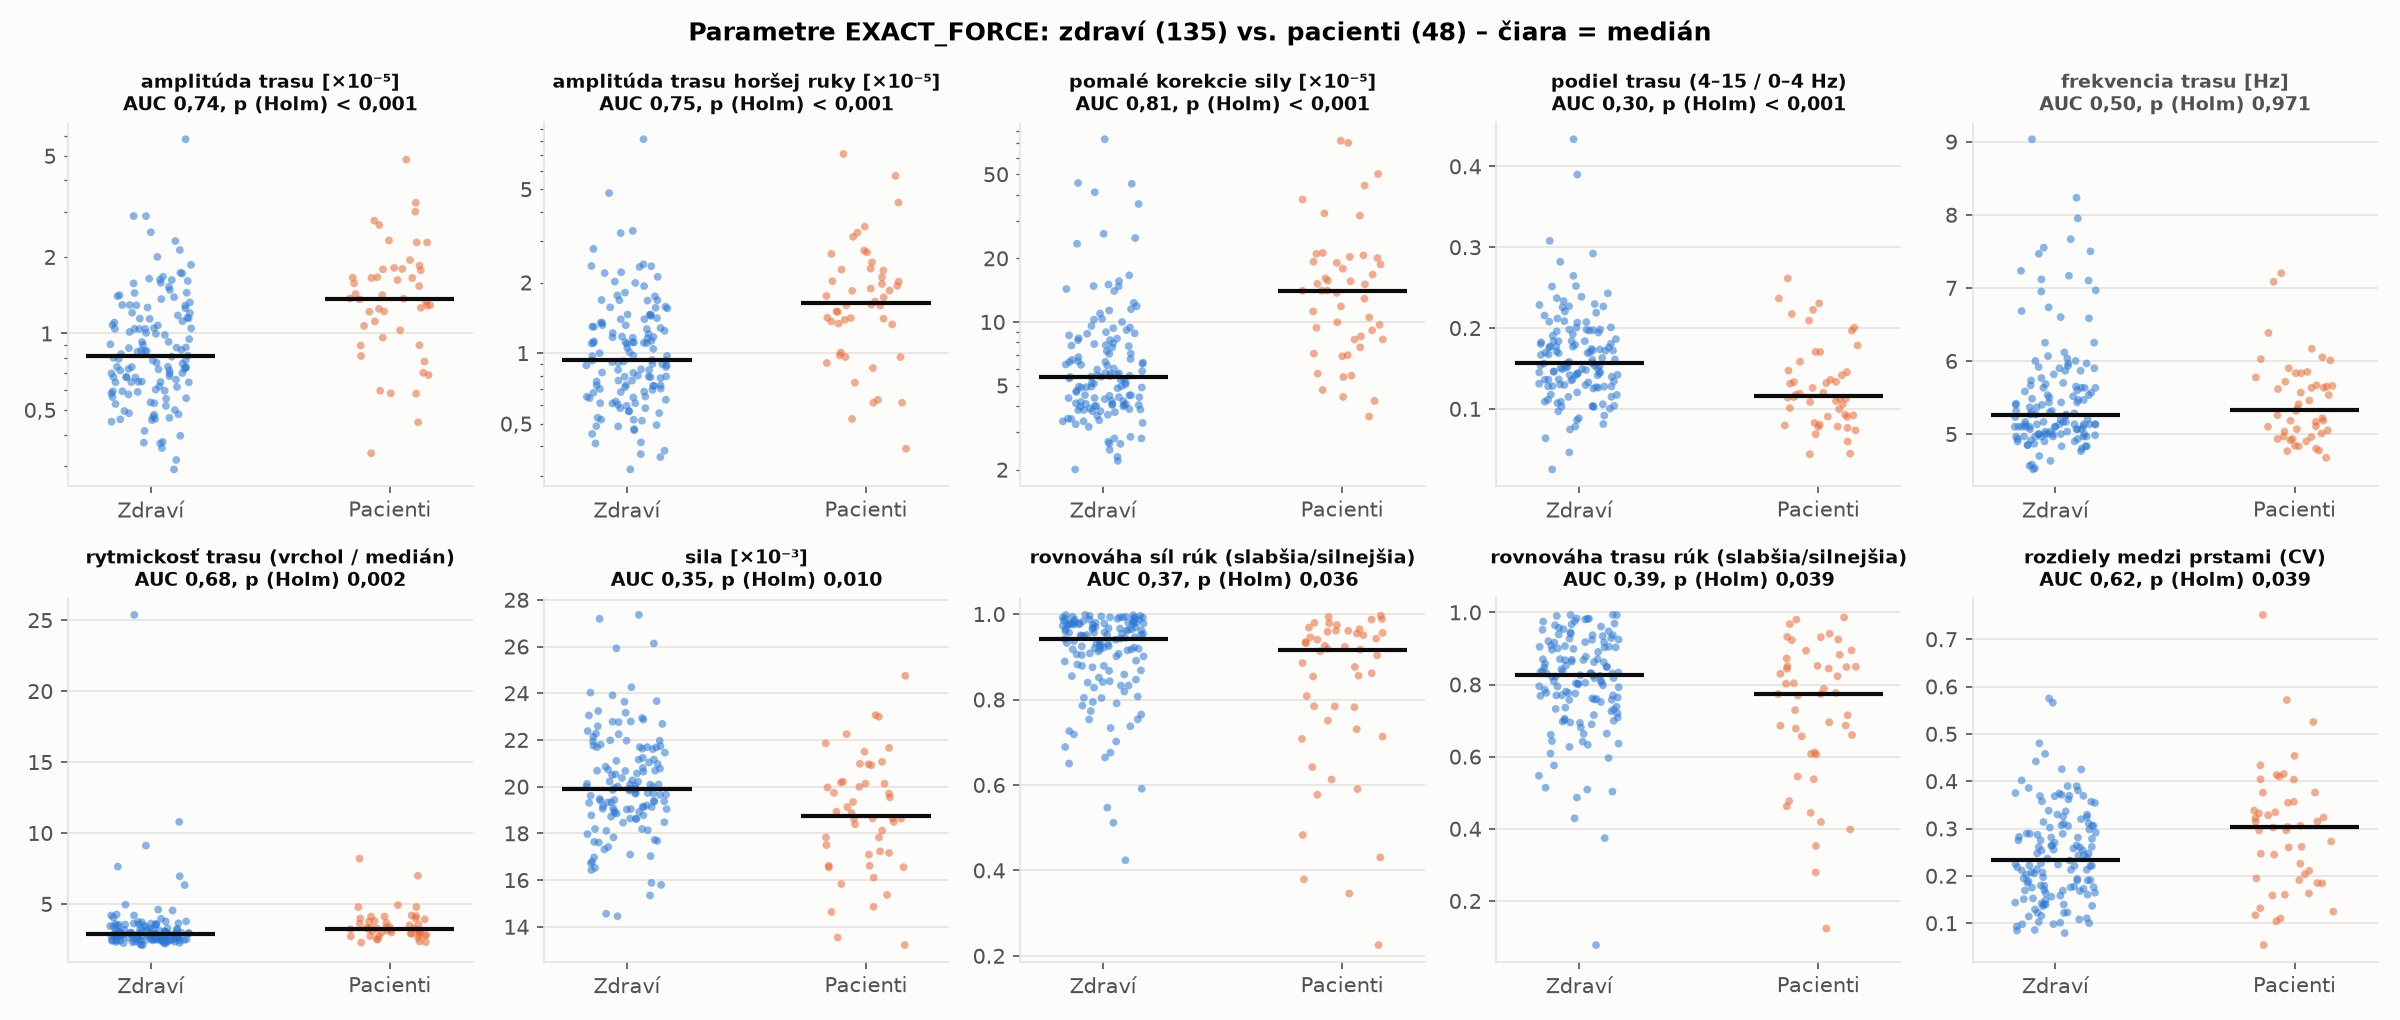
\includegraphics[width=\textwidth]{ef_parametre.png}
\caption{\ef{}: bod = osoba, čiara = medián skupiny. Čierny nadpis = významný rozdiel (krok 1).}
\end{figure}

\subsection{Vek a normy}
\begin{itemize}
  \item S~vekom sa po Holmovej korekcii menia štyri parametre: \textbf{podiel trasu} ($\rho = -0{,}27$) a~\textbf{frekvencia
        trasu} ($\rho = -0{,}27$) klesajú, \textbf{rytmickosť trasu} ($\rho = 0{,}36$) a~\textbf{sila} ($\rho = 0{,}26$)
        stúpajú. Trendy sú slabé a~čiastočne môžu byť rozdielom miest merania (starší zdraví sú väčšinou z~meracieho
        centra). Amplitúda trasu, pomalé korekcie a~rovnováha rúk od veku nezávisia.
  \item Normy (medián [2,5 -- 97,5\,\%]) a~počet pacientov mimo normy:
\end{itemize}

\begin{table}[H]
\centering
\small
\begin{tabular}{lll}
\toprule
parameter & norma & pacienti mimo normy \\
\midrule
podiel trasu -- 20 -- 29 rokov & 0,169 [0,102 -- 0,301] & \textbf{10 z~48} mimo normy svojej dekády \\
podiel trasu -- 70 -- 79 rokov & 0,138 [0,076 -- 0,232] & \\
sila -- 20 -- 29 rokov [$\times 10^{-3}$] & 19,5 [15,4 -- 23,2] & \textbf{10 z~48} mimo normy (9 pod) \\
sila -- 70 -- 79 rokov [$\times 10^{-3}$] & 20,7 [17,0 -- 25,9] & \\
rovnováha síl rúk & 0,941 [0,612 -- 0,996] & 7 pod, 1 nad normou \\
amplitúda trasu [$\times 10^{-5}$] & 0,82 [0,37 -- 2,44] & 5 nad, 1 pod normou \\
rozdiely medzi prstami & 0,232 [0,095 -- 0,452] & 4 nad, 1 pod normou \\
pomalé korekcie sily [$\times 10^{-5}$] & 5,49 [2,54 -- 39,4] & 4 nad normou \\
\bottomrule
\end{tabular}
\end{table}

Parametre s~vplyvom veku (podiel trasu, frekvencia, rytmickosť, sila) majú normu podľa veku (kvantilová regresia),
ostatné jednu normu pre všetky dekády. Pomalé korekcie sily majú u~niektorých starších zdravých veľké hodnoty, preto
je ich horná hranica široká a~nad ňou je len 4 z~48 pacientov, hoci je to parameter s~najväčším rozdielom skupín.

\subsection{Klasifikátor a ablácia}
\begin{itemize}
  \item Logistická regresia z~parametrov \ef{}: \textbf{AUC 0,77} (citlivosť 0,66, špecificita 0,78);
        s~vekom 0,82; len vek 0,64; len osoby nad 50 rokov 0,84. Náhodný les 0,77. Permutačný test $p = 0{,}005$.
  \item Ablácia: najsilnejší faktor sám sú \textbf{pomalé korekcie sily} (AUC 0,81), potom amplitúda trasu (0,74).
        Po vynechaní jedného faktora AUC klesne najviac o~0,012 (sila) -- faktory sa navzájom zastupujú.
        S~vekom v~modeli je vek faktor s~najväčším poklesom (0,049).
\end{itemize}

\begin{figure}[H]
\centering
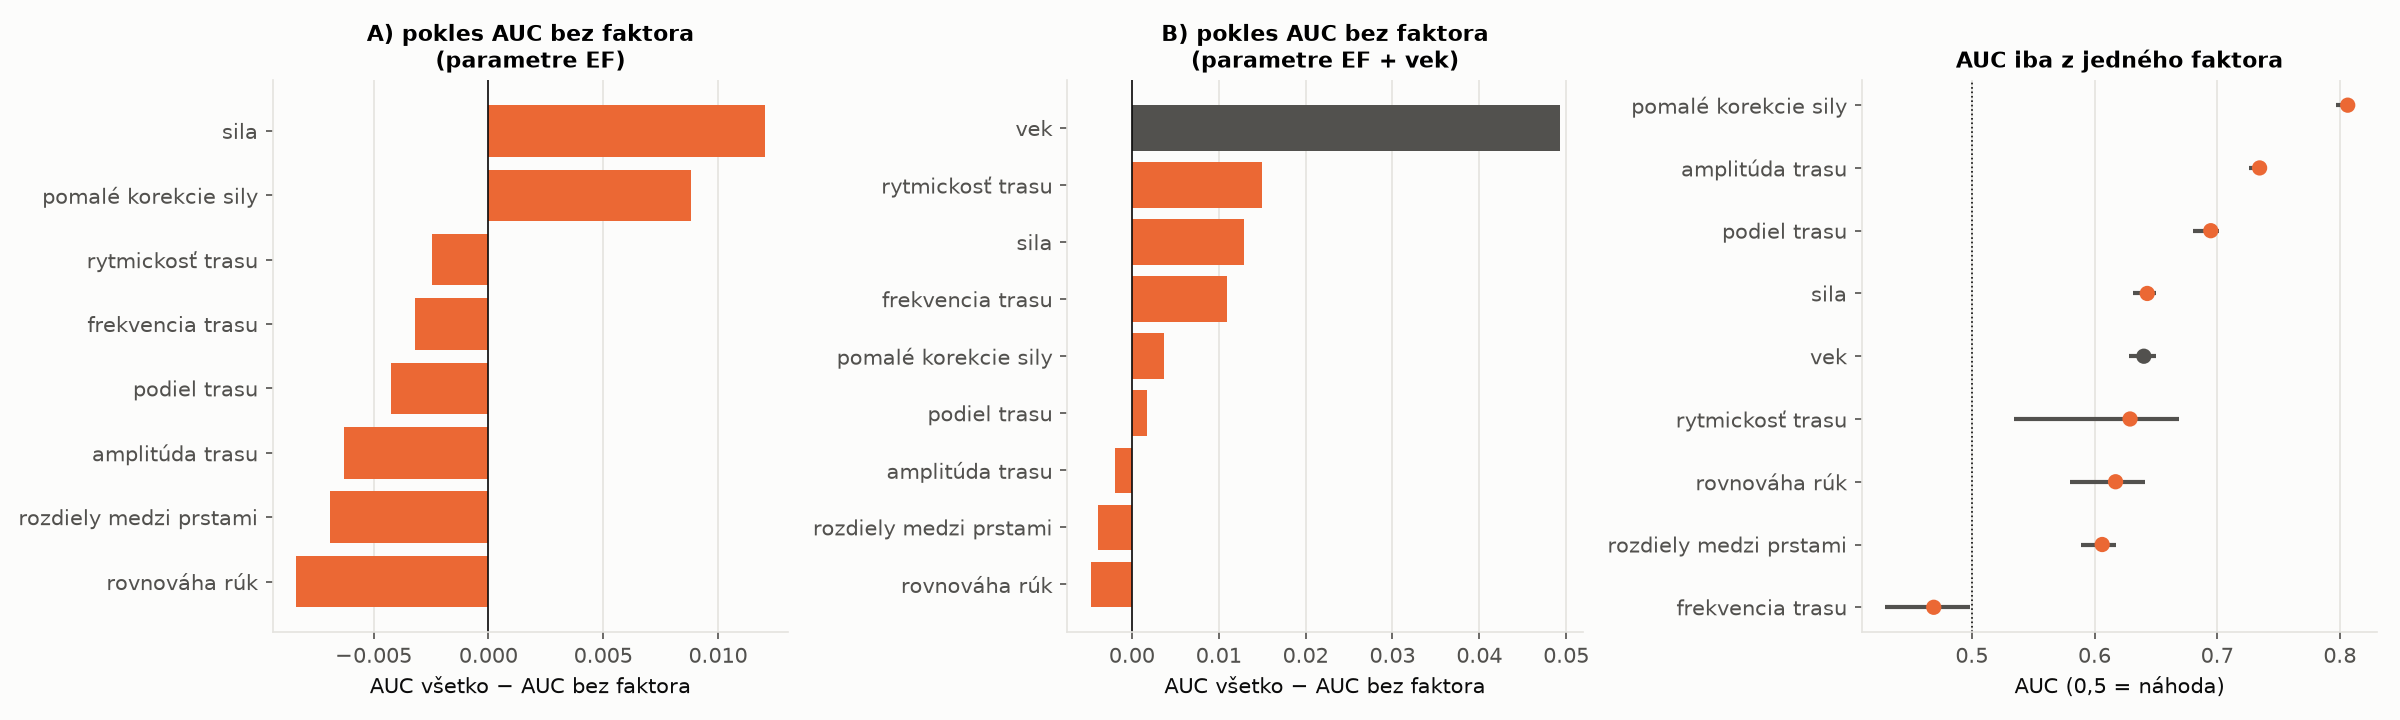
\includegraphics[width=\textwidth]{ef_ablacia.png}
\caption{\ef{} -- ablácia: pokles AUC bez faktora (A -- parametre, B -- parametre + vek) a~AUC iba z~jedného faktora.}
\end{figure}

% ===================================================================================================
\section{Rytmický test}

\subsection{Spracovanie}
\begin{enumerate}
  \item Sila ruky = priemer jej 5 snímačov. Analyzuje sa úsek 2 -- 30~s pokusu.
  \item \textbf{Stlačenia} = vrcholy súčtu síl oboch rúk (\texttt{scipy.signal.find\_peaks}): vrchol musí byť
        aspoň 0,25~s od predchádzajúceho a~vyčnievať aspoň o~25\,\% rozsahu sily pokusu. Stlačenie = úsek od minima
        pred vrcholom po minimum za ním. Pokus s~menej ako 5 stlačeniami sa nepoužije.
        Časy stlačení, ktoré ukladá hra, nesedia so signálom sily (korelácia od $-0{,}55$ do $+0{,}70$), preto sa
        nepoužívajú.
  \item \textbf{1. pokus sa nepoužíva} -- je nácvik (ľudia v~ňom stláčajú pomalšie a~silnejšie).
  \item Hodnota osoby = medián pokusov 2 -- 4 jedného merania, potom priemer meraní osoby.
\end{enumerate}

\subsection{Hypotézy a výsledky}

\begin{table}[H]
\centering
\small
\caption{Rytmický test: parametre, hypotézy (H1 -- u~pacientov je parameter \dots) a~výsledok.}
\begin{tabularx}{\textwidth}{l L l l}
\toprule
faktor & parameter (čo meria) & H1 & výsledok \\
\midrule
tempo & počet stlačení za sekundu & nižší & \yes \\
pravidelnosť rytmu & rozptyl intervalov medzi stlačeniami / ich priemer & vyšší & \no \\
sila stlačenia & veľkosť stlačenia silnejšej ruky & nižší & opačný smer, len bez kontroly veku \\
 & veľkosť stlačenia slabšej ruky & nižší & \no \\
rovnováha rúk & slabšia ruka / silnejšia ruka (1 = rovnaké) & nižší & \yes{} (všetky kroky) \\
stálosť sily & rozptyl veľkosti stlačení / ich priemer & vyšší & \no \\
súčasnosť rúk & časový rozdiel vrcholu ľavej a~pravej ruky & vyšší & \yes \\
uvoľnenie & sila po stlačení / sila vo vrchole & vyšší & opačný smer, len bez kontroly veku \\
únava & sila v~2. / 1. polovici pokusu & nižší & \no \\
 & tempo v~2. / 1. polovici pokusu & nižší & \no \\
\bottomrule
\end{tabularx}
\end{table}

\begin{table}[H]
\centering
\small
\caption{Rytmický test: medián a p-hodnota po Holmovej korekcii v~každom kroku (\ok{} = $p < 0{,}05$).}
\setlength{\tabcolsep}{4.5pt}
\begin{tabular}{lcccccc}
\toprule
parameter & zdraví & pacienti & 1. všetci & 2. rovn. vek & 3. model + vek & 4. + tempo \\
\midrule
rovnováha rúk & 0,838 & 0,699 & \ok{} $<0{,}001$ & \ok{} 0,002 & \ok{} $<0{,}001$ & \ok{} $<0{,}001$ \\
tempo [stlačení/s] & 2,46 & 1,63 & \ok{} $<0{,}001$ & \ok{} 0,005 & \ok{} $<0{,}001$ & -- \\
oneskorenie rúk [ms] & 20 & 30 & \ok{} $<0{,}001$ & \ok{} 0,010 & 0,052 & 0,089 \\
sila silnejšej ruky & 0,069 & 0,084 & \ok{} 0,016 & 0,307 & \ok{} 0,041 & 0,649 \\
neúplné uvoľnenie & 0,165 & 0,086 & \ok{} 0,010 & 0,221 & 0,136 & 0,649 \\
stálosť sily (CV) & 0,158 & 0,147 & 1,000 & 0,823 & 0,603 & \ok{} 0,027 \\
pravidelnosť, sila slabšej ruky, & & & & & & \\
\quad únava (2) & & & n.s. & n.s. & n.s. & n.s. \\
\bottomrule
\end{tabular}
\end{table}

\textbf{Interpretácia:}
\begin{itemize}
  \item \textbf{Rovnováha rúk} je najspoľahlivejší rozdiel -- zostáva vo všetkých štyroch krokoch. Pacientom jedna
        ruka tlačí výrazne slabšie a~nie je to vekom ani pomalším tempom.
  \item \textbf{Tempo:} pacienti stláčajú pomalšie (približne 1,6 vs. 2,5 stlačenia za sekundu), aj pri rovnakom veku.
  \item \textbf{Oneskorenie rúk} je významné pri porovnaní v~dekádach, nie však v~lineárnom modeli. Model pokazí
        niekoľko pacientov s~veľmi veľkým oneskorením (120 -- 510~ms); test v~dekádach pracuje s~poradím hodnôt
        a~je voči nim odolný.
  \item \textbf{Opačný smer:} pacienti tlačia silnejšou rukou \textbf{silnejšie} a~ruky \textbf{úplnejšie uvoľnia}.
        Je to dôsledok pomalšieho tempa -- kto stláča pomaly, stihne ruku úplne uvoľniť a~stlačiť silnejšie.
        Po pridaní tempa do modelu ani jedno nie je významné a~v~dekádach sa tiež nelíšia.
  \item \textbf{Stálosť sily} sa líši len pri rovnakom tempe (krok 4): pri rovnakej rýchlosti stláčania kolíše
        pacientom veľkosť stlačení viac.
\end{itemize}

\begin{figure}[H]
\centering
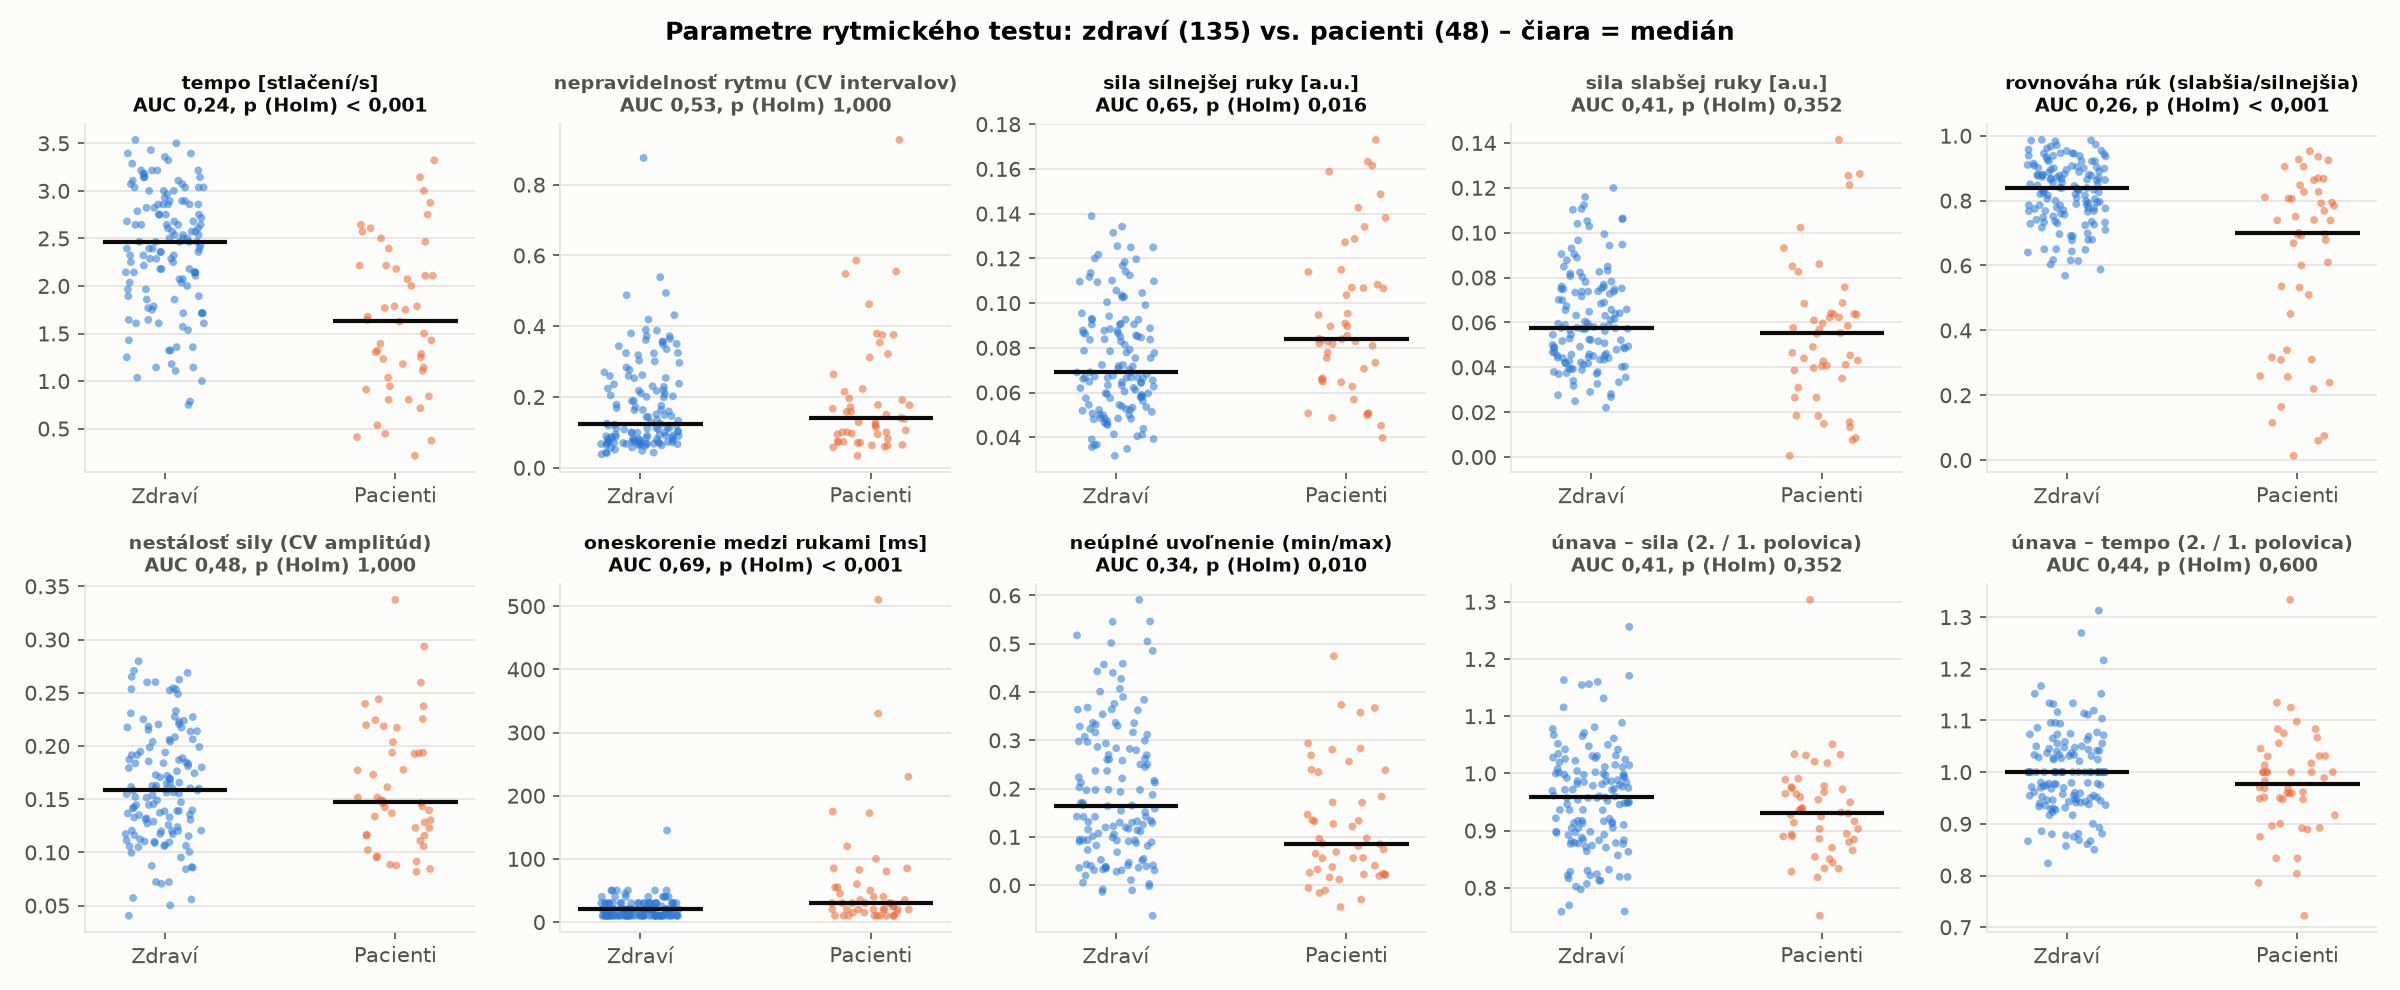
\includegraphics[width=\textwidth]{rytmus_parametre.png}
\caption{Rytmický test: bod = osoba, čiara = medián skupiny. Čierny nadpis = významný rozdiel (krok 1).}
\end{figure}

\subsection{Vek a normy}
\begin{itemize}
  \item S~vekom sa po Holmovej korekcii menia štyri parametre -- všetky klesajú: \textbf{tempo} ($\rho = -0{,}32$),
        \textbf{nepravidelnosť rytmu} ($\rho = -0{,}44$), \textbf{nestálosť sily} ($\rho = -0{,}46$) a~\textbf{neúplné
        uvoľnenie} ($\rho = -0{,}34$). Starší zdraví stláčajú pomalšie, ale pravidelnejšie. Časť trendu môže byť
        rozdielom miest merania (mladí z~TUKE, starší väčšinou z~meracieho centra).
  \item \textbf{Rovnováha rúk od veku nezávisí} ($\rho = -0{,}09$) -- jej pokles u~pacientov je prejavom
        ochorenia, nie starnutia. Norma rovnováhy je spoločná pre všetky dekády, tempo a~uvoľnenie majú normu
        podľa veku:
\end{itemize}

\begin{table}[H]
\centering
\small
\begin{tabular}{lll}
\toprule
parameter & norma: medián [2,5 -- 97,5\,\%] & pacienti mimo normy \\
\midrule
rovnováha rúk & 0,838 [0,615 -- 0,979] & \textbf{19 z~48} pod normou \\
oneskorenie rúk [ms] & 20 [10 -- 50] & 14 nad normou \\
tempo -- 20 -- 29 rokov [stlačení/s] & 2,63 [1,29 -- 3,39] & 10 pod normou svojho veku \\
tempo -- 70 -- 79 rokov [stlačení/s] & 2,25 [0,75 -- 3,39] & \\
sila silnejšej ruky & 0,069 [0,037 -- 0,125] & 10 nad normou \\
neúplné uvoľnenie -- 20 -- 29 / 70 -- 79 rokov & 0,249 / 0,097 & 4 pod normou svojho veku \\
\bottomrule
\end{tabular}
\end{table}

Mimo normy je z~definície aj 5\,\% zdravých, preto hodnota mimo normy ešte neznamená ochorenie.

\subsection{Klasifikátor a ablácia}
\begin{itemize}
  \item Logistická regresia z~parametrov rytmu: \textbf{AUC 0,81} (citlivosť 0,70, špecificita 0,79); s~vekom 0,82;
        len vek 0,64; len osoby nad 50 rokov 0,80. Náhodný les 0,76. Permutačný test $p = 0{,}005$.
  \item Ablácia: najviac prispievajú \textbf{tempo} (sám AUC 0,75, bez neho pokles 0,025), \textbf{rovnováha rúk}
        (0,74; pokles 0,014) a~\textbf{sila stlačenia} (0,74). Pravidelnosť, stálosť sily a~únava samy dávajú len
        0,42 -- 0,57. Poklesy sú malé, lebo parametre sa navzájom zastupujú; rovnováha rúk nesie informáciu, ktorú
        ostatné parametre nemajú. S~vekom v~modeli je vek faktor s~najväčším poklesom (0,016).
\end{itemize}

\begin{figure}[H]
\centering
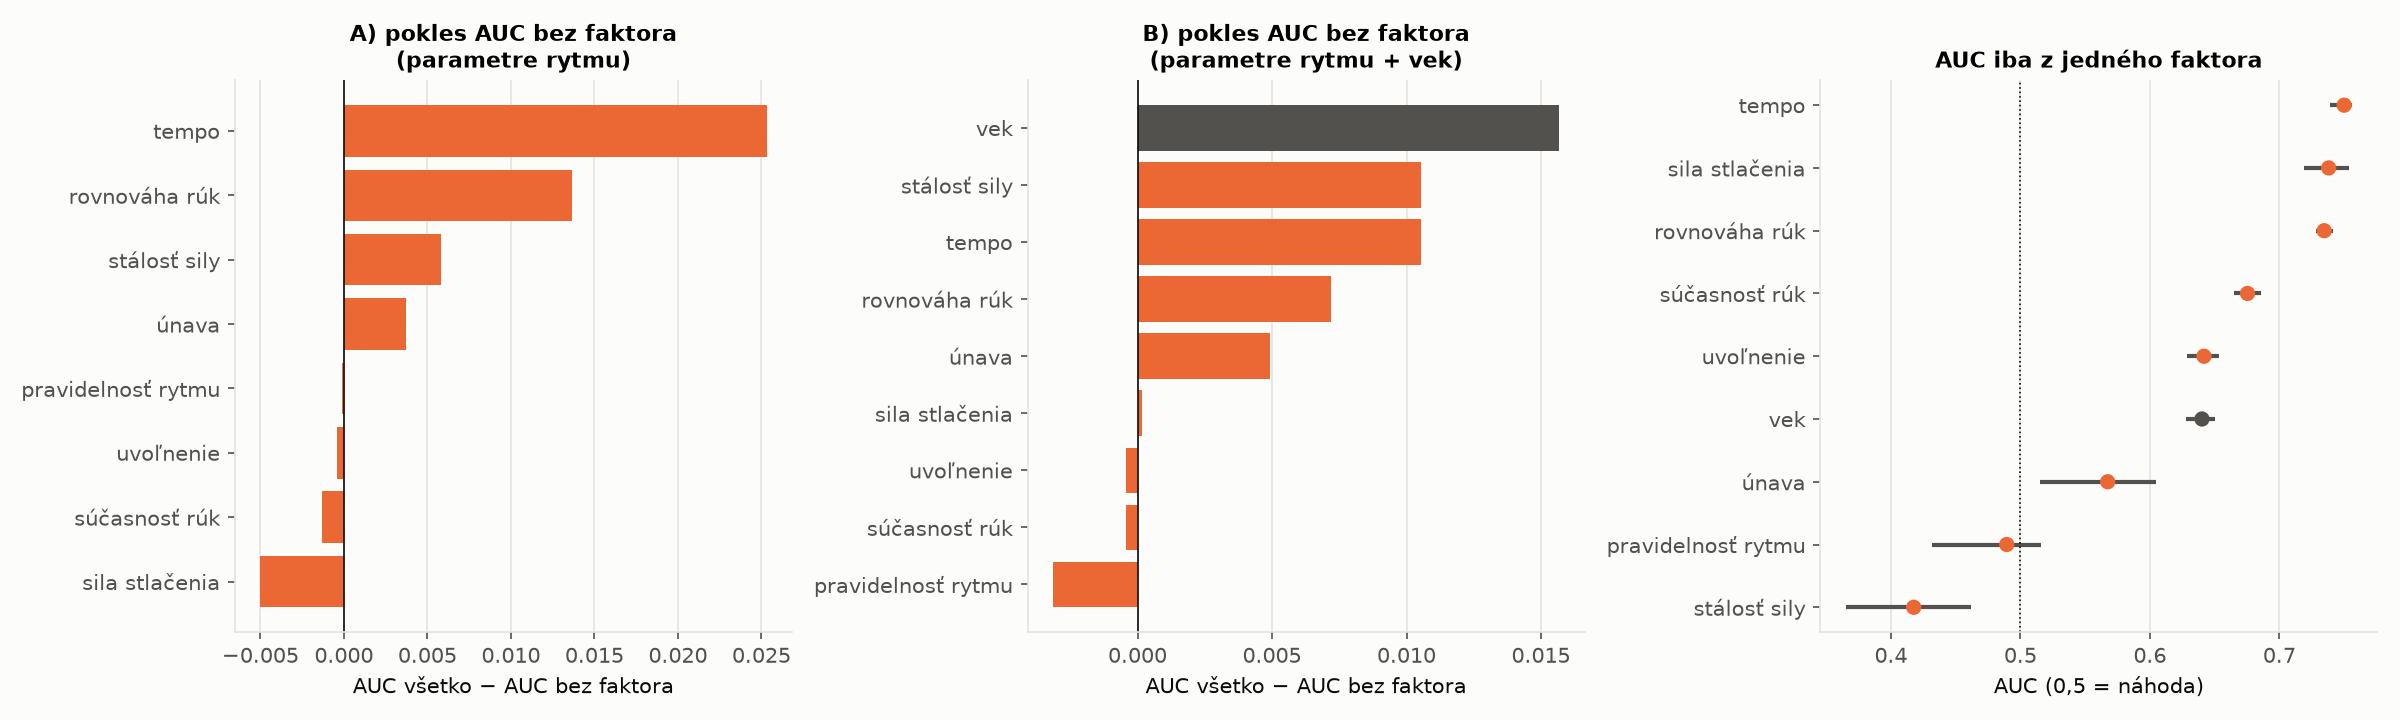
\includegraphics[width=\textwidth]{rytmus_ablacia.png}
\caption{Rytmický test -- ablácia: pokles AUC bez faktora (A -- parametre, B -- parametre + vek) a~AUC iba
z~jedného faktora.}
\end{figure}

% ===================================================================================================
\section{Porovnanie testov \ef{} a rytmus}

Kód \path{src/rehapiano/comparison.py}, notebook \path{notebooks/combined/porovnanie_exact_force_rytmus.ipynb}.

\begin{table}[H]
\centering
\small
\caption{Závery oboch testov vedľa seba.}
\begin{tabularx}{\textwidth}{l L L}
\toprule
 & \ef{} & rytmus \\
\midrule
čo meria & tras a~stabilitu držanej sily & rýchlosť, koordináciu, rovnováhu rúk \\
potvrdené hypotézy (rovnaký vek) & pomalé korekcie sily, amplitúda trasu (aj horšej ruky), sila prstov
  & tempo, rovnováha rúk, súčasnosť rúk \\
opačný smer, ako sme čakali & podiel trasu & sila silnejšej ruky, uvoľnenie (len bez kontroly veku) \\
najsilnejší parameter (AUC) & pomalé korekcie sily (0,81) & tempo (0,76) \\
mení sa s~vekom u~zdravých & podiel trasu, frekvencia a~rytmickosť trasu, sila & tempo, pravidelnosť, stálosť sily,
  uvoľnenie \\
rovnováha rúk: pacienti pod normou & 7 z~48 & 19 z~48 \\
klasifikátor (AUC) & 0,77 & 0,81 \\
opakovateľnosť (medián ICC) & 0,56 & 0,65 \\
\bottomrule
\end{tabularx}
\end{table}

\begin{table}[H]
\centering
\small
\caption{Logistická regresia, AUC: každý test zvlášť a oba testy spolu.}
\begin{tabular}{lccc}
\toprule
príznaky & \ef{} & rytmus & oba testy \\
\midrule
parametre testu & 0,77 & 0,81 & 0,85 \\
parametre + vek & 0,82 & 0,82 & 0,86 \\
len vek & 0,64 & 0,64 & 0,64 \\
len osoby nad 50 rokov & 0,84 & 0,80 & 0,86 \\
\bottomrule
\end{tabular}
\end{table}

\textbf{Zistenia:}
\begin{enumerate}
  \item \textbf{Oba testy oddelia pacientov podobne dobre (rytmus o~niečo lepšie), ale podľa iných prejavov.}
        Test \ef{} podľa nestabilnej sily, trasu a~menšej sily, rytmický test podľa spomalenia, nerovnováhy
        a~nesúčasnosti rúk.
  \item \textbf{Slabšiu ruku ukáže lepšie rytmický test.} V~\ef{} sa rovnováha rúk pri rovnakom veku nelíši
        ($p = 0{,}19$), v~rytme áno ($p = 0{,}002$). Všetkých 7 pacientov pod normou v~\ef{} je pod normou
        aj v~rytme, rytmus nájde ďalších 12. Pri pokojnom držaní sily stačí slabšej ruke malá sila; rýchle opakované
        stláčanie ju viac zaťaží.
  \item \textbf{Testy nemerajú to isté.} Korelácie parametrov medzi testami sú u~zdravých takmer nulové
        (medián $|\rho| = 0{,}06$), u~pacientov slabé (medián $|\rho| = 0{,}17$, najviac 0,49). Kto je postihnutý
        viac, býva horší v~oboch testoch, ale každý test zachytí iné vlastnosti pohybu.
  \item \textbf{Testy sa dopĺňajú.} Z~48 pacientov rozpoznajú oba klasifikátory 25, len \ef{} 8, len rytmus 8,
        žiadny 7. Aspoň jeden test zachytí 41 z~48 pacientov (každý sám 33). Pravdepodobnosti oboch klasifikátorov
        u~pacientov súvisia len stredne ($\rho = 0{,}41$). Priemer pravdepodobností oboch testov dáva AUC 0,86,
        spoločný model zo všetkých 20 parametrov 0,85; medzi rovnako starými (nad 50 rokov) oba testy spolu 0,86,
        kým každý sám 0,80 -- 0,84.
  \item \textbf{Rytmický test je opakovateľnejší.} U~35 pacientov meraných dvakrát
        (\textbf{ICC} = zhoda 1. a~2. merania; 1 = rovnaké hodnoty, nad 0,75 dobrá, pod 0,5 slabá):
  \begin{itemize}
    \item rytmus: rovnováha rúk 0,87, tempo 0,76, sila stlačenia 0,77 -- 0,80;
    \item \ef{}: rytmickosť trasu 0,85, podiel trasu 0,77, ale sila prstov 0,25 a~amplitúda trasu 0,54;
    \item únava v~rytme sa nezopakuje vôbec (ICC približne 0) -- preto ani neoddeľuje skupiny;
    \item oneskorenie rúk má ICC 0,17 kvôli jednému pacientovi (950~ms a~potom 70~ms), poradie pacientov sa však
          zachová ($\rho = 0{,}83$);
    \item po Holmovej korekcii sa pri 2. meraní žiadny parameter významne nezmenil.
  \end{itemize}
\end{enumerate}

\begin{figure}[H]
\centering
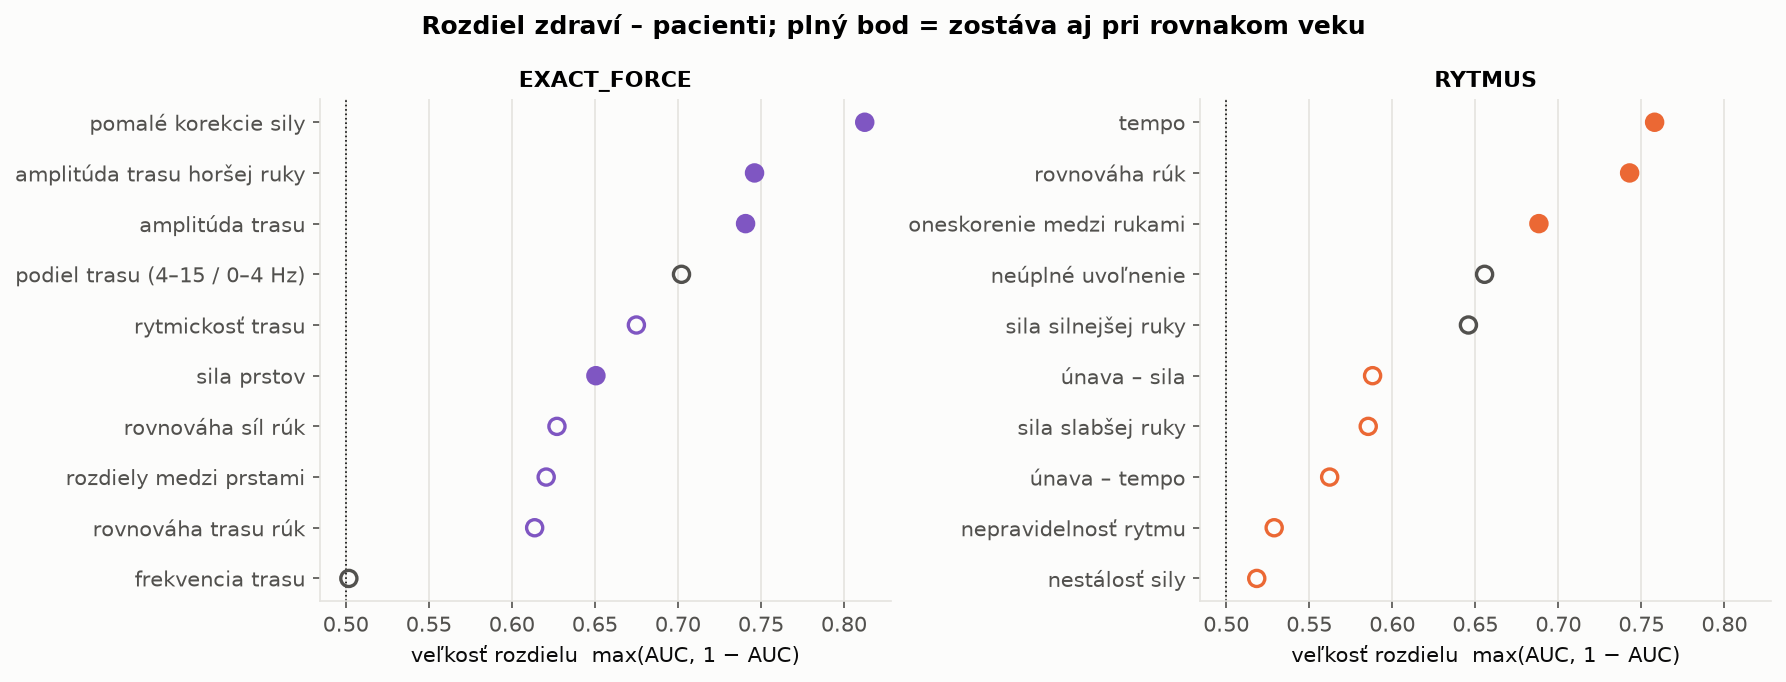
\includegraphics[width=\textwidth]{porovnanie_rozdiely.png}
\caption{Veľkosť rozdielu zdraví -- pacienti pre všetkých 20 parametrov; plný bod = rozdiel zostáva aj pri rovnakom
veku, sivá = opačný smer, ako sme čakali.}
\end{figure}

\begin{figure}[H]
\centering
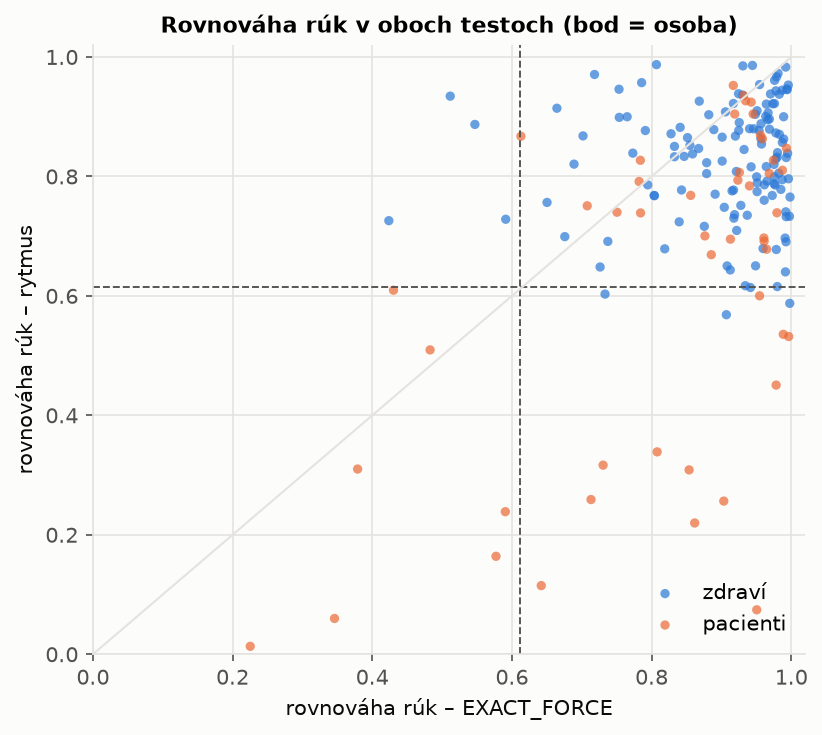
\includegraphics[width=0.46\textwidth]{porovnanie_rovnovaha.png}\hfill
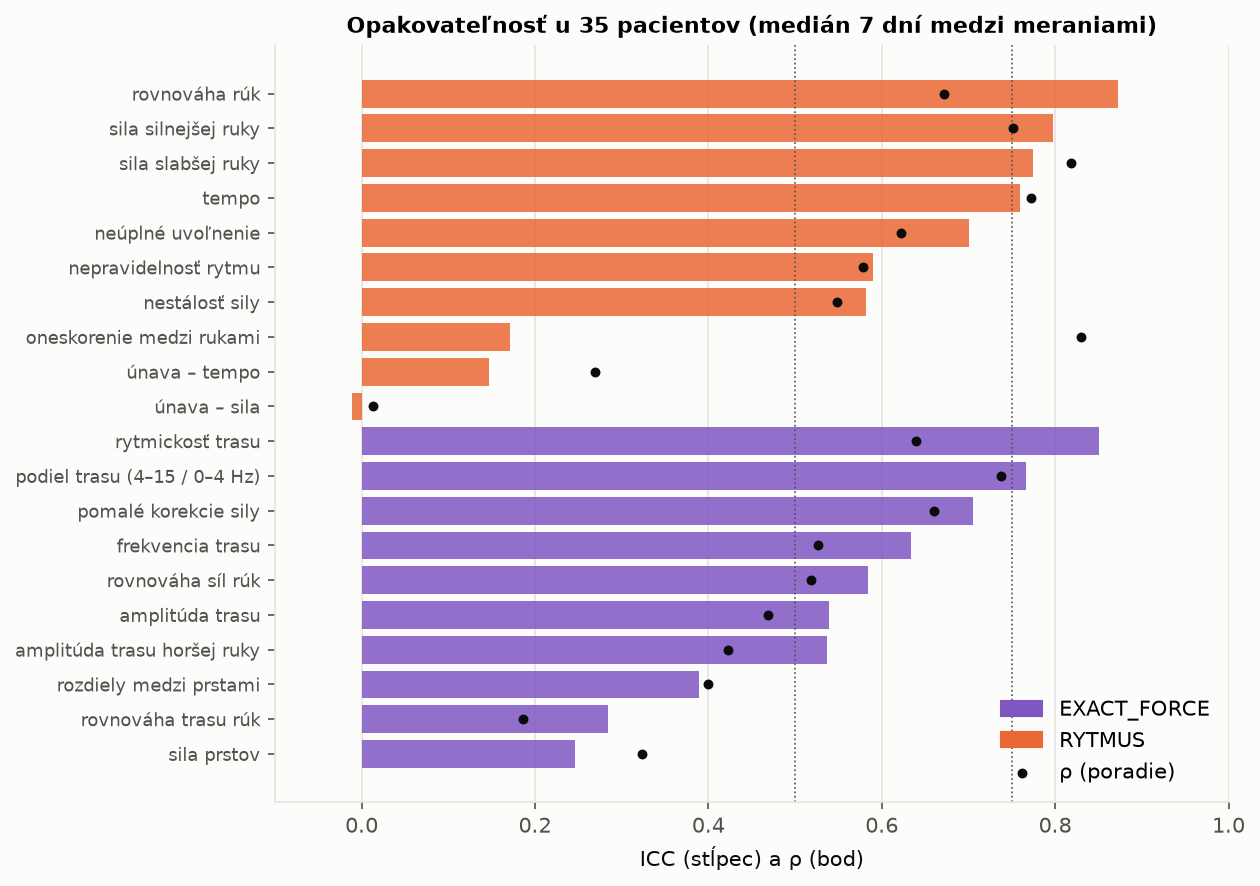
\includegraphics[width=0.52\textwidth]{porovnanie_opakovatelnost.png}
\caption{Vľavo: rovnováha rúk v~oboch testoch (čiarkované = dolná hranica normy). Vpravo: opakovateľnosť
parametrov u~35 pacientov (stĺpec = ICC, bod = $\rho$).}
\end{figure}

% ===================================================================================================
\section{Diskusia}

\begin{itemize}
  \item \textbf{Hlavný výsledok:} pacienti sa od zdravých líšia aj pri rovnakom veku -- v~\ef{}
        \textbf{nestabilnou silou}, \textbf{trasom} a~menšou silou prstov, v~rytme \textbf{pomalším tempom},
        \textbf{nerovnováhou} a~\textbf{nesúčasnosťou rúk}. Oba testy sú dôležité: každý zachytí iných pacientov
        a~spolu sú lepšie ako ktorýkoľvek sám.
  \item \textbf{Vek už nie je hlavný rušivý faktor.} S~74 zdravými nad 50 rokov (pred meraním v~centre ich bolo 17)
        sú skupiny vekovo podobné (medián 61 vs. 66,5 rokov) a~len vek oddelí skupiny s~AUC 0,64. Výsledky pri rovnakom
        veku sú preto oveľa presnejšie ako predtým. Zostáva však \textbf{miesto merania}: mladí zdraví sú z~TUKE,
        starší väčšinou z~meracieho centra, takže zmeny s~vekom u~zdravých môžu byť čiastočne rozdielom miest.
  \item \textbf{Verzia úlohy:} zdraví a~pacienti hrali v~oboch testoch inú verziu hry (iné \texttt{step\_id}).
        Časť rozdielu, napr. v~tempe, môže byť spôsobená verziou hry. Porovnanie v~dekádach odstráni vek,
        nie verziu hry.
  \item \textbf{Opačné smery majú vysvetlenie:} v~rytme silnejšie stlačenie a~úplnejšie uvoľnenie vyplývajú
        z~pomalšieho tempa; v~\ef{} je podiel trasu nižší, lebo pomalé kolísanie sily rastie viac ako tras.
  \item \textbf{Normy:} pre parametre s~vplyvom veku (v~\ef{} štyri, v~rytme štyri) sa hranice menia s~vekom, pre
        ostatné je jedna norma. Spoľahlivé (aspoň 20 zdravých) sú dekády 20 -- 29, 60 -- 69 a~70 -- 79; v~dekádach
        30 -- 59 a~nad 80 rokov je zdravých stále málo. Mimo normy je z~definície aj 5\,\% zdravých.
  \item \textbf{Sledovanie pacienta v~čase:} najvhodnejšie sú opakovateľné parametre -- rovnováha rúk a~tempo
        v~rytme. Amplitúda trasu a~sila v~\ef{} sa medzi dňami menia viac. Opakovateľnosť máme len pre pacientov;
        medzi meraniami mohla prebiehať liečba.
  \item \textbf{Klasifikátor nie je diagnostický nástroj} -- nie je overený na nezávislých dátach.
\end{itemize}

\textbf{Odporúčania:} namerať zdravých vo veku 30 -- 59 a~nad 80 rokov (aspoň 20 v~dekáde), časť mladých zdravých
zmerať aj v~meracom centre (aby sa dal oddeliť vplyv veku od miesta merania), doplniť metadáta nových pacientov
z~roku 2026, používať jednu verziu hry pre všetkých, zmerať zdravých dvakrát a~overiť klasifikátor na nových osobách.

% ===================================================================================================
\section{Kde čo nájsť}

\begin{table}[H]
\centering
\footnotesize
\begin{tabularx}{\textwidth}{L l}
\toprule
čo & kde \\
\midrule
\ef{} -- hypotézy, normy, klasifikátor, ablácia & \path{notebooks/exact_force/statisticka_analyza_exact_force.ipynb} \\
rytmus -- rovnováha rúk & \path{notebooks/rhythm/rovnovaha_ruk.ipynb} \\
rytmus -- hypotézy, normy, klasifikátor, ablácia & \path{notebooks/rhythm/statisticka_analyza_rytmus.ipynb} \\
klasifikátor z~oboch testov & \path{notebooks/combined/klasifikator_oba_testy.ipynb} \\
hypotézy a~normy po dekádach & \path{notebooks/combined/hypotezy_a_normy.ipynb} \\
porovnanie testov & \path{notebooks/combined/porovnanie_exact_force_rytmus.ipynb} \\
parametre \ef{} & \path{src/rehapiano/exact_force/parameters.py} \\
detekcia stlačení a~parametre rytmu & \path{src/rehapiano/rhythm/presses.py}, \path{parameters.py} \\
štatistika, klasifikátor, ablácia & \path{src/rehapiano/common/stats/group_analysis.py} \\
porovnanie testov & \path{src/rehapiano/comparison.py} \\
tabuľky výsledkov & \path{outputs/exact_force/analysis/}, \path{outputs/rhythm/analysis/}, \path{outputs/comparison/} \\
\bottomrule
\end{tabularx}
\end{table}

Celý projekt sa prepočíta príkazom \texttt{python scripts/run\_all.py} (s~\texttt{-{}-notebooks} aj notebooky).

% ---------------------------------------------------------------------------------------------------
\section*{Slovník pojmov}

\begin{table}[H]
\centering
\small
\begin{tabularx}{\textwidth}{l L}
\toprule
pojem & význam \\
\midrule
p-hodnota & pravdepodobnosť takého alebo väčšieho rozdielu, keby v~skutočnosti žiadny rozdiel nebol;
  $p < 0{,}05$ $\Rightarrow$ H0 zamietame \\
Holmova korekcia & oprava p-hodnôt pri viacerých testoch naraz: najmenšia p $\times$ počet testov,
  ďalšia $\times$ (počet $-$ 1) \dots \\
Mann-Whitneyho test & porovnanie dvoch skupín podľa poradia hodnôt, nepotrebuje normálne rozdelenie \\
van Elterenov test & Mann-Whitney v~každej dekáde zvlášť, spojený do jedného testu -- porovnáva rovnako starých \\
AUC & 0,5 = skupiny sa neodlišujú, 1 = úplne oddelené; pri klasifikátore plocha pod ROC krivkou \\
Spearmanovo $\rho$ & sila súvislosti dvoch veličín podľa poradia: 0 = žiadna, $\pm 1$ = úplná \\
spektrogram & rozklad signálu na frekvencie v~čase; pásmo 4 -- 15~Hz = tras, 0 -- 4~Hz = pomalé korekcie sily \\
krížová validácia & model sa hodnotí vždy na osobách, ktoré pri učení nevidel \\
ICC & zhoda dvoch meraní tých istých ľudí: 1 = rovnaké hodnoty, nad 0,75 dobrá, pod 0,5 slabá \\
ablácia & vynechanie jednej skupiny parametrov z~modelu, aby sme zistili, koľko prispieva \\
\bottomrule
\end{tabularx}
\end{table}

\end{document}
